\subsection{Supervised learning} \label{sec:supervised}

\mode<presentation>{

\begin{frame}{\secname:~\subsecname}

\begin{center}
\begin{minipage}{0.4\textwidth}
\begin{center}
	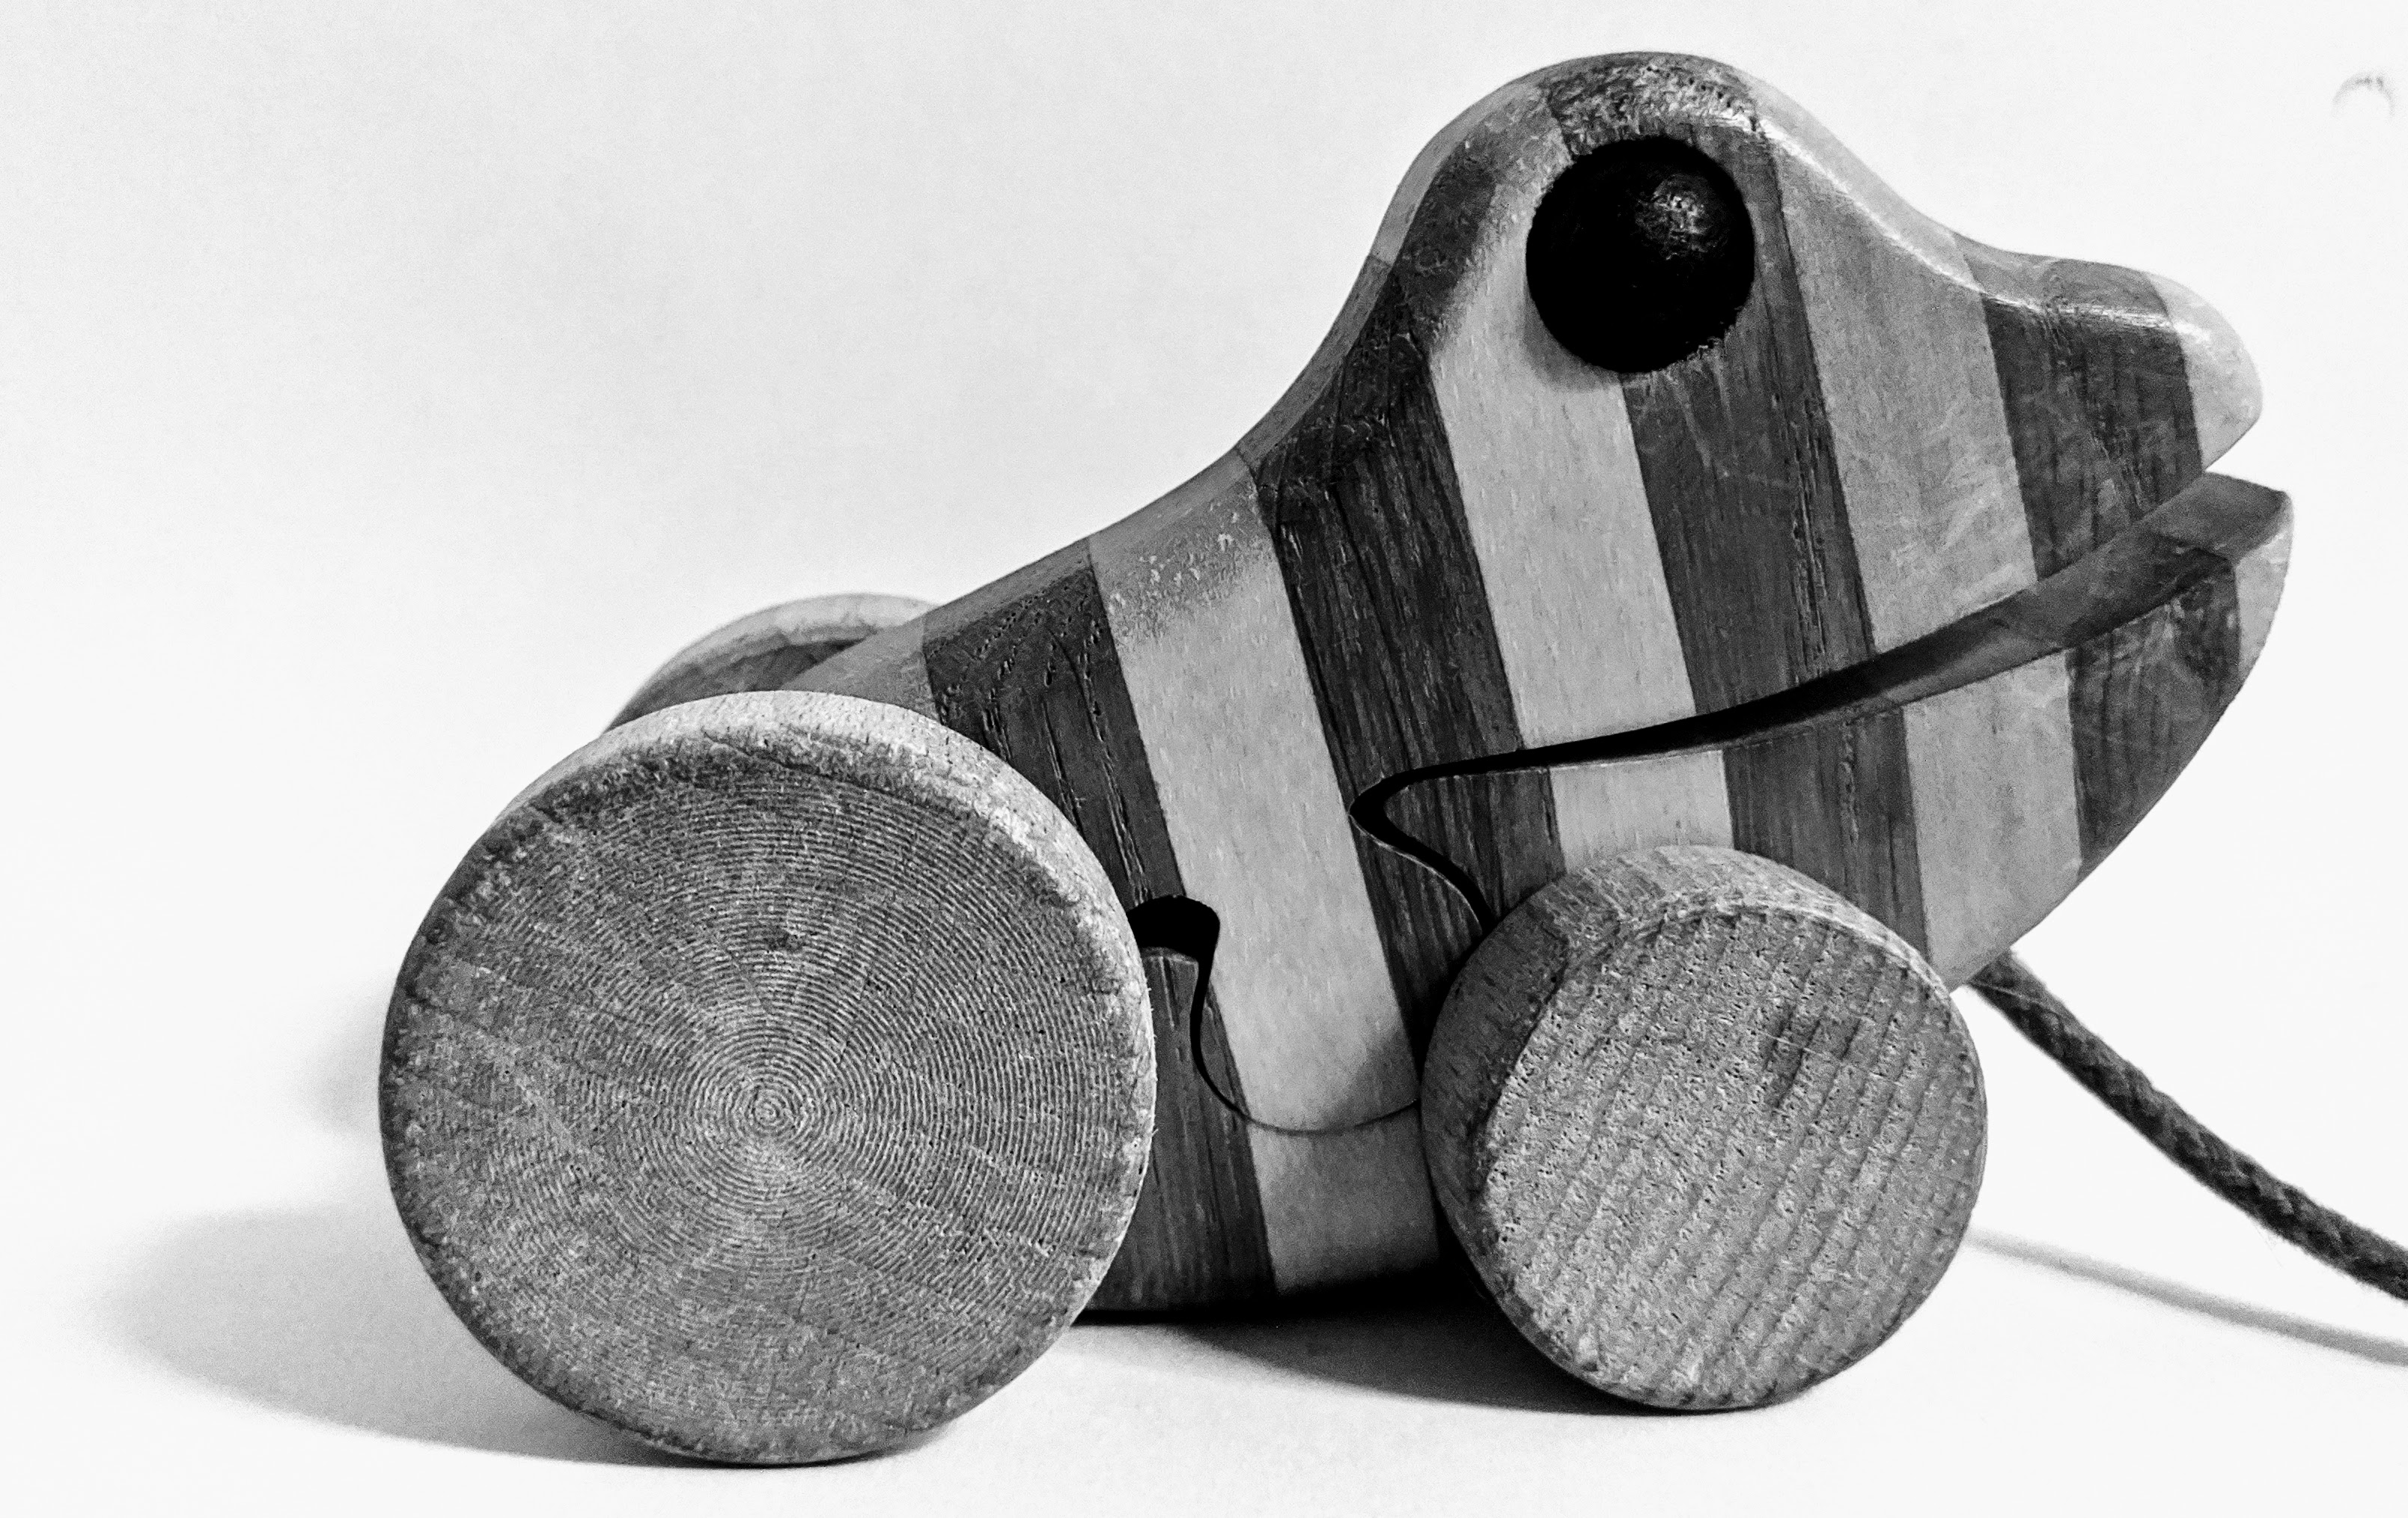
\includegraphics[height=3cm]{img/tigerente}
	\captionof*{figure}{example image recognition}
\end{center}
\end{minipage}
\hspace{1cm}
\begin{minipage}{0.4\textwidth}
\begin{center}
	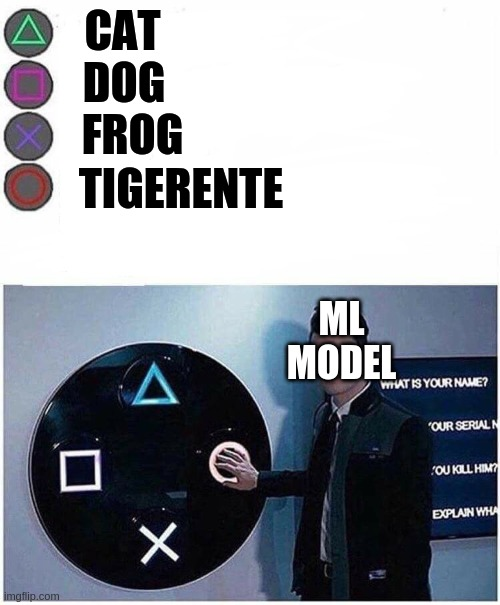
\includegraphics[height=4cm]{img/meme_choose}
\end{center}
\end{minipage}
\end{center}

\vspace{10mm}

%Is it a:\\
%cat, dog, tiger, duck, frog or fish?

\end{frame}
}

\begin{frame}{\secname:~\subsecname}

We are given data that is made up of tuples.

Supervised methods try to fit a function that maps $\vec x$ to some attribute $\vec y$ (labels/ground truth).

\begin{center}
	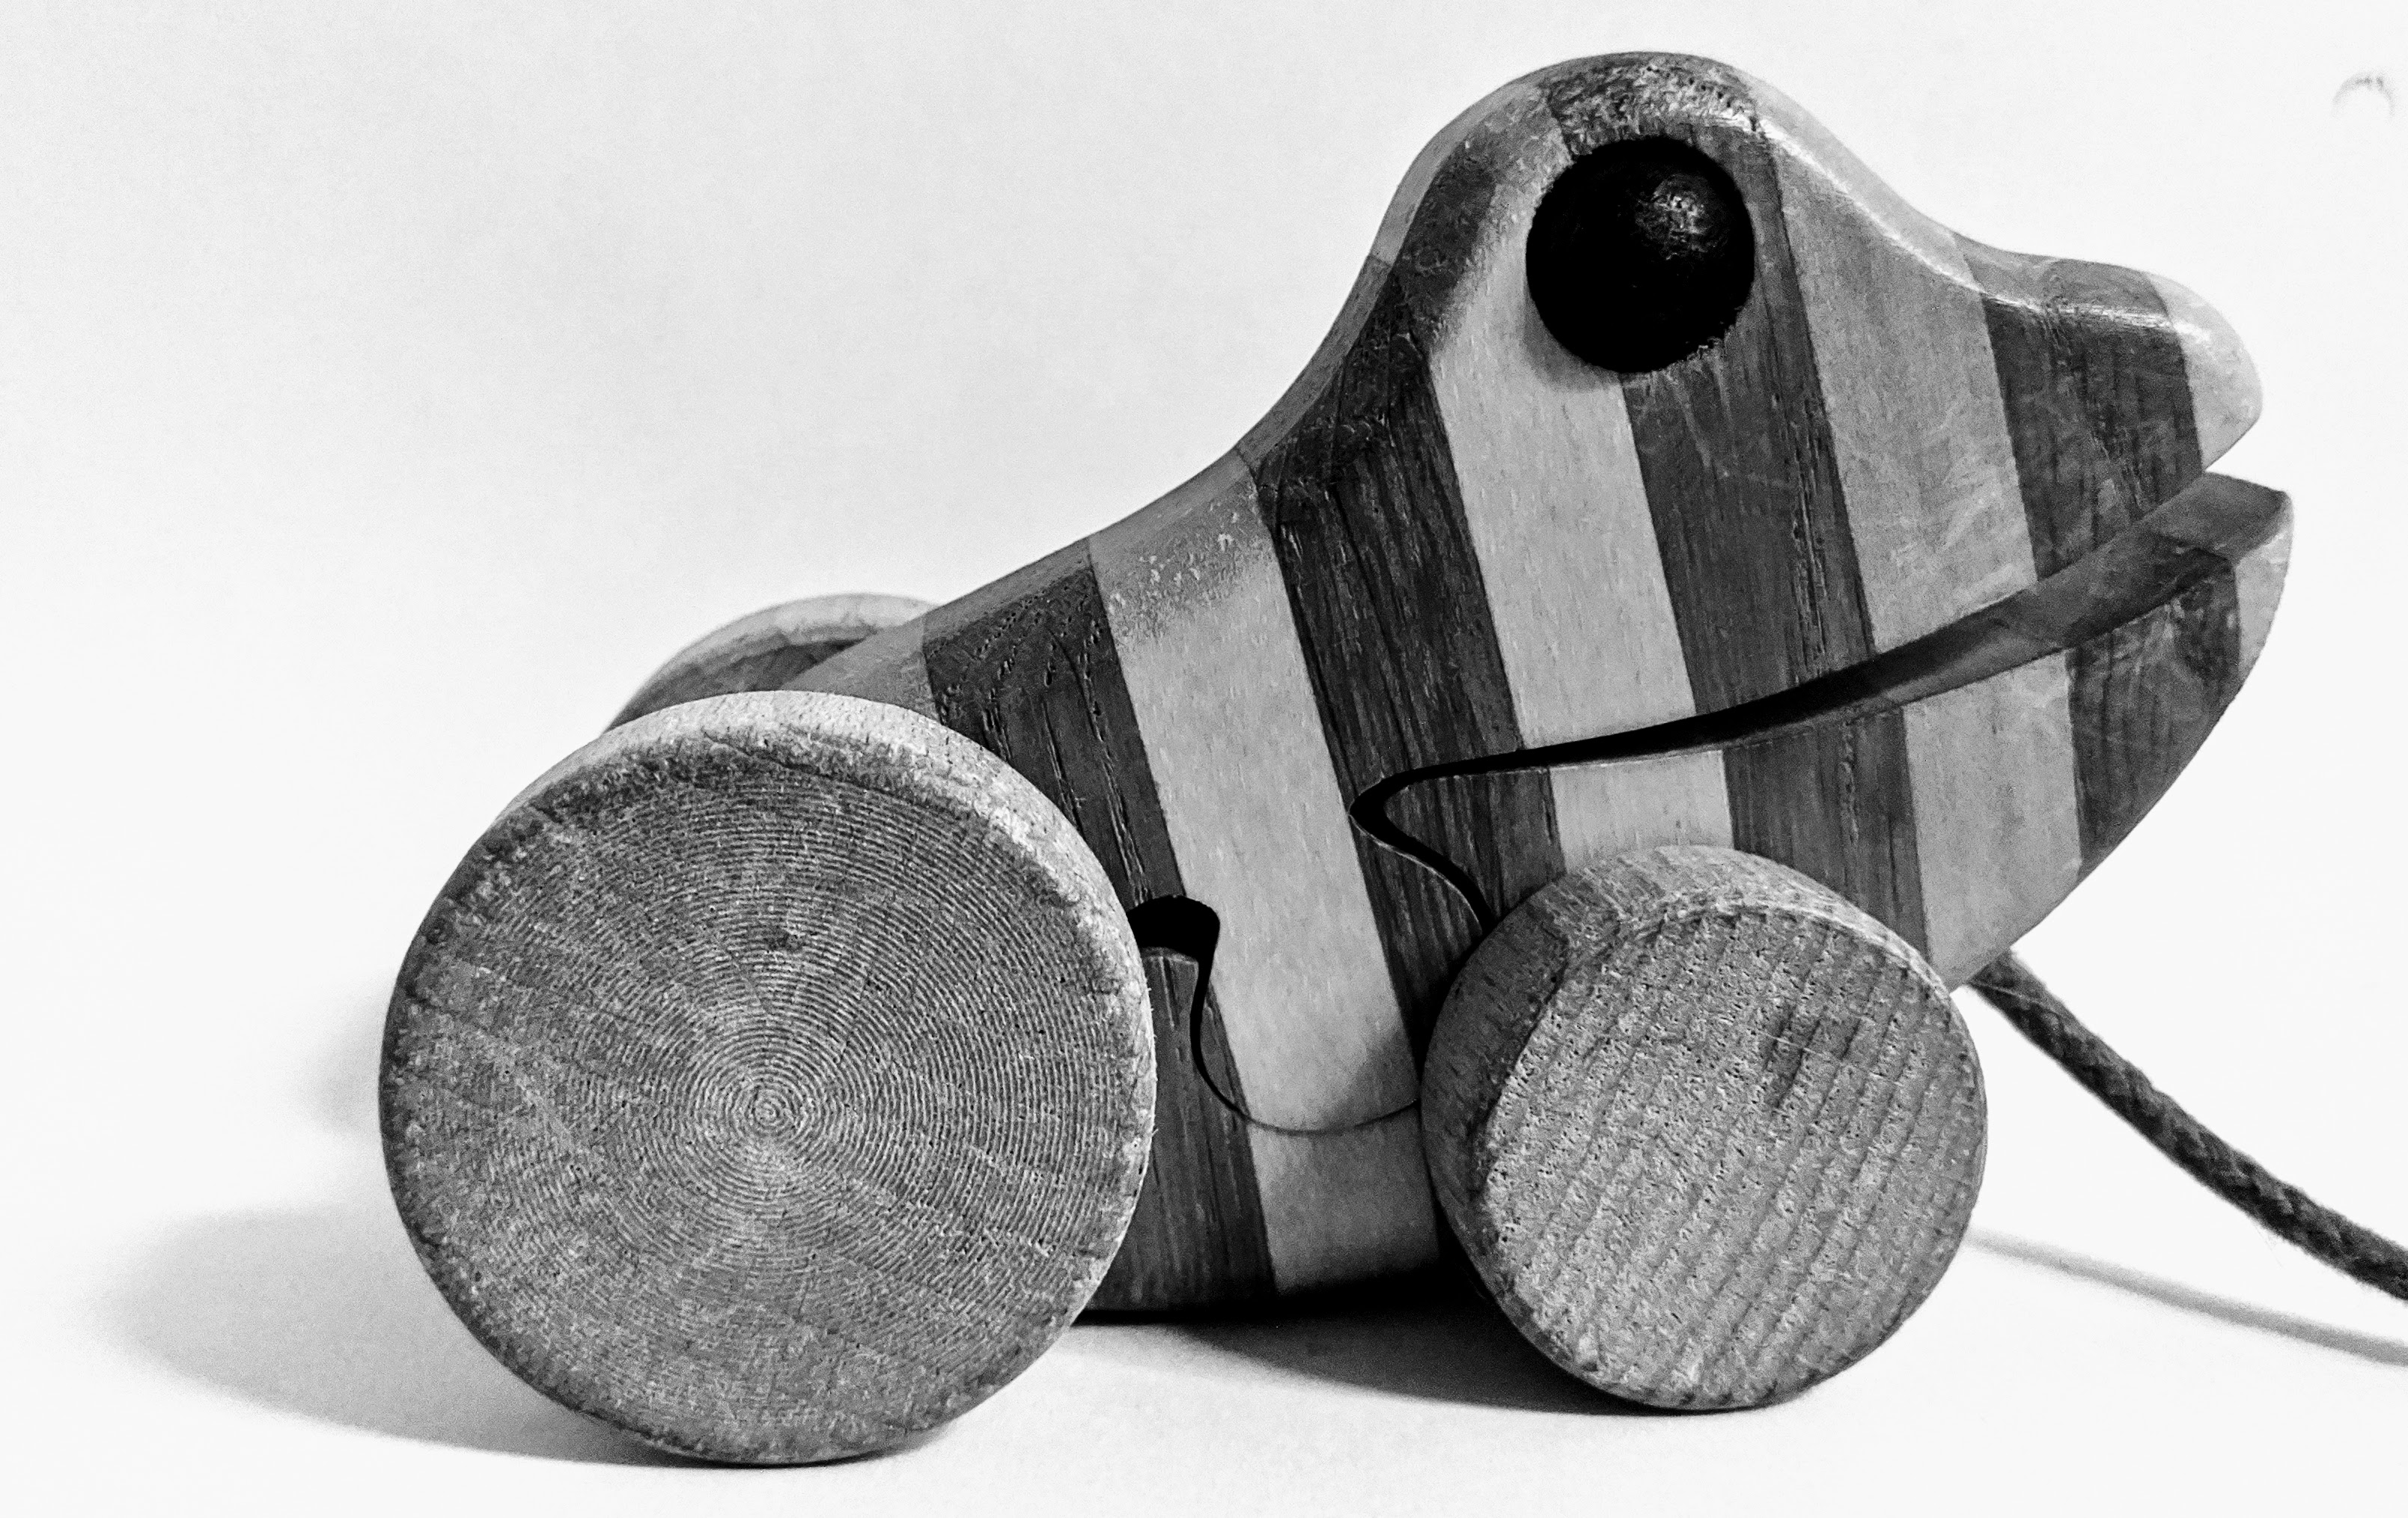
\includegraphics[height=2cm]{img/tigerente}
	\captionof*{figure}{example image recognition}
\end{center}

Supervised learning would fit a function that maps image pixels to recognizing the object in the image\\
from a set of possible objects (e.g. cat, dog, tiger, duck, frog, fish).
    
\end{frame}

\begin{frame}\frametitle{\subsecname}

\mode<article>Supervised learning is\mode<all>essentially function fitting.

\underline{Data}:\\
\mode<presentation>{\vspace{5mm}}

Consider this dataset of tuples:
\begin{equation}
\label{eq:tuples}
\left( \vec x^{(1)}, \vec y_T^{(1)} \right) \,,\, \ldots \,,\, \left( \vec x^{(\alpha)}, \vec y_T^{(\alpha)} \right) \,,\, \ldots \,,\, \left( \vec x^{(p)}, \vec y_T^{(p)} \right)
\end{equation}

\mode<article>{
where,
\begin{itemize}
\item[] $\vec x$ denotes the observation with $N$ components. $\vec x = (x_1, x_2, \ldots x_N)$, $\vec x \in \R^N$ (e.g. pixel values in an image)
\item[] $\vec y_T$ denotes the label assigned to this observation. It is also referred to as the ground truth.
When $y_T \in \R$ or $\vec y_T \in \R^M$, we are looking at a regression problem (e.g. predicting house prices, object localization - bounding box regression (x, y, w, h)).\\
When $y_T \in \{ 0, 1\}$, we refer to this as a binary classification problem (e.g. is this a cat or a dog).\\
When $y_T \in \{ 0, \ldots, K-1\}$, we refer to this as a multi-class classification problem (e.g. which letter is this?).
\item[] $p$ denotes the size of the dataset (i.e. how many labeled observations we have.)
\item[] The superscript $^{(\alpha)}$ denotes the index of a particular sample within the dataset. $\alpha = 1 , \ldots, p$
\item[] The samples are often assumed to be \emph{independent and identically distributed} (\iid).
\end{itemize}
}

%\end{frame}
\pause
%\begin{frame}

\underline{Objective model}:\\
\mode<presentation>{\vspace{5mm}}
\notesonly{Supervised learning algorithms are used to }find a function that maps observations to their label(s)\notesonly{ which represents some concept or value.
This mapping can be described in the form of:}
\begin{itemize}
\item a discriminative function $\vec y = \vec f(\vec x)$, \\ 

\notesonly{
where $\vec f(\cdot)$ denotes a vector valued function }$\vec f: \R^N \rightarrow \R^M$
\item a conditional distribution $P(\,\vec y \,|\, \vec x\,)$.
\end{itemize}

\end{frame}


